\documentclass[screen,review]{thesis}

%% The cover page lives in cover.sty, loaded here, with its metadata
%% in frontmatter/cover.tex. Redefine \maketitle to change the layout.
\usepackage{cover}
\title{A Study of Something Interesting}
\subtitle{Towards a Better Understanding of the Problem}

\author{Jane Q. Doe}
\affiliation{Department of Computer Science\\University of Somewhere\\Somewhere, Country}
% \email{jane.doe@example.edu}
\orcid{0000-0000-0000-0000}
% \authornote{Corresponding author.}

\degree{Doctor of Philosophy}
\supervisor{Prof. Ada Lovelace}
\cosupervisor{Dr. Alan Turing}
\submissiondate{October 2026}

%% ---- Typography (optional) ------------------------------------------
%% The text face is a class option:
%%   \documentclass[print,font=times]{thesis}   (also font=palatino)
%% and the base size is 14pt by default (also 10/11/12/17/20pt).
%% Adjust the running head, heading sizes, line spacing or paragraph
%% spacing with a single setup command. Headings are serif by default;
%% add \sffamily to a heading value for sans-serif headings.
% \thesissetup{
%   head       = {\small},
%   chapter    = {\bfseries\LARGE},
%   section    = {\bfseries\Large},
%   subsection = {\bfseries\large},
%   linespread = 1.15,
%   parskip    = 6pt,
% }
%% ---------------------------------------------------------------------

\begin{document}

\frontmatter
\maketitle

\cleardoublepage\thispagestyle{empty}\null\vspace{\stretch{1}}%
\begin{center}
    \textit{ To everyone who asked ``is it done yet?'' --- almost.}
\end{center}
\vspace{\stretch{2}}\null
\begin{frontchapter}[Declaration]
I hereby declare that this thesis is my own work and that it has not been
submitted for any other degree or qualification. All sources of
information have been acknowledged by means of references.

\vspace{1cm}

\noindent\rule{5cm}{0.2pt} \\
\noindent
\theauthor\\
\thesubmissiondate
\end{frontchapter}

\begin{frontchapter}[Preface]
This thesis grew out of a simple question that turned out to be far from
simple. This preface records the motivation and the scope of the work,
and explains how the chapters fit together.

The structure is as follows. Chapter~\ref{ch:overview} reviews the
template styles and parameters, Chapter~\ref{ch:elements} describes the
document elements, Chapter~\ref{ch:floats} covers tables and figures,
Chapter~\ref{ch:math} mathematics, and Chapter~\ref{ch:citations}
citations and bibliographies. Chapter~\ref{ch:conclusion} concludes.

\end{frontchapter}
\begin{frontchapter}{Acknowledgements}
I am grateful to my supervisor, Prof. Ada Lovelace, for her patient
guidance, and to Dr. Alan Turing for many stimulating discussions. Thanks
also go to my colleagues and family for their support.
\end{frontchapter}

\begin{abstract}
This thesis investigates an interesting problem and proposes a method to
address it. We present a formal treatment, an implementation, and an
empirical evaluation. The results show that the proposed method improves
upon the state of the art on standard benchmarks.
\end{abstract}

\tableofcontents
\listoffigures
\listoftables

\mainmatter
\chapter{Introduction}
\label{ch:introduction}

ACM's consolidated article template, introduced in 2017, provides a
consistent \LaTeX\ style for use across ACM publications, and
incorporates accessibility and metadata-extraction functionality
necessary for future Digital Library endeavors. Numerous ACM and
SIG-specific \LaTeX\ templates have been examined, and their unique
features incorporated into this single new template.

This thesis template builds on that work. Where the ACM template is a
single article, this document is arranged by chapter and provides the
usual parts of a thesis: a cover page, a table of contents, lists of
figures and tables, an abstract, the main chapters, a bibliography, and
special parts such as the declaration, preface and acknowledgements.

If you are new to \LaTeX, this document doubles as a guide to preparing
your thesis. If you have used the ACM template before, it shows how its
features map onto the structure of a thesis.

\section{Outline}
\label{sec:outline}

Chapter~\ref{ch:overview} reviews the template styles and parameters.
Chapter~\ref{ch:elements} describes the document elements, from
typefaces to sectioning. Chapter~\ref{ch:floats} covers tables and
figures, Chapter~\ref{ch:math} mathematics, and Chapter~\ref{ch:citations}
citations and bibliographies. Chapter~\ref{ch:conclusion} concludes.

\chapter{Template Overview}
\label{ch:overview}

As noted in the introduction, this document class can be used to prepare
many different renderings of the same thesis --- a copy for review, a
clean copy for printing and binding, and a copy for reading on screen ---
all by selecting the appropriate {\itshape template style} and {\itshape
  template parameters}.

This document explains the major features of the document class. For
further information on the original ACM class, the {\itshape \LaTeX\
User's Guide} is available from
\url{https://www.acm.org/publications/proceedings-template}.

\section{Template Styles}
\label{sec:styles}

The primary parameter given to the document class is the {\itshape
  template style}, which corresponds to the intended use of the output.
This parameter is enclosed in square brackets and is a part of the
\verb|documentclass| command:
\begin{verbatim}
  \documentclass[STYLE]{thesis}
\end{verbatim}

The thesis template defines three styles:
\begin{itemize}
\item {\texttt{print}}: a two-sided (duplex) copy with binding margins,
  suitable for printing and binding. This is the default.
\item {\texttt{screen}}: a one-sided copy for reading on screen, with
  coloured hyperlinks.
\item {\texttt{review}}: a one-sided reading copy with line numbers.
\end{itemize}

\section{Template Parameters}
\label{sec:parameters}

In addition to specifying the {\itshape template style}, there are a
number of {\itshape template parameters} which modify some part of the
applied template style. The base font size is 14\,pt by default, and
10, 11, 12, 17 and 20\,pt are also accepted. Frequently-used parameters
include:
\begin{itemize}
\item {\texttt{onehalf}}, {\texttt{double}}: line spacing.
\item {\texttt{font=times}}: a Times-like text face ({\texttt{font=libertine}}
  is the default).
\item {\texttt{authoryear}}: author--year citations.
\item {\texttt{biblatex}}: use \BibLaTeX\ with the \texttt{acmnumeric}
  or \texttt{acmauthoryear} styles instead of \BibTeX.
\end{itemize}


Testing the listing
\begin{itemize}
  \item Something
  \item Another one
\end{itemize}

This document uses the following string as the first command in the
source file:
\begin{verbatim}
\documentclass[print]{thesis}
\end{verbatim}

\section{Files and Building}
\label{sec:files}

The template is built with the usual \LaTeX\ tools. With \texttt{latexmk}:
\begin{verbatim}
  latexmk -pdf thesis.tex
\end{verbatim}
or, manually, \verb|pdflatex|, then \verb|bibtex|, then \verb|pdflatex|
twice more. A full \TeX\ Live (or MiKTeX) installation is required; the
class uses the standard packages \texttt{extsizes}, \texttt{libertine},
\texttt{newtxmath}, \texttt{geometry}, \texttt{titlesec},
\texttt{fancyhdr}, \texttt{setspace}, \texttt{natbib}, \texttt{hyperref},
\texttt{microtype}, \texttt{booktabs}, \texttt{amsmath} and
\texttt{amsthm}.

The entry point is \texttt{thesis.tex}, and the files are laid out as
follows:
\begin{verbatim}
  thesis.cls   the thesis class (structure, typography)
  cover.sty    the cover page
  thesis.tex      entry point
  frontmatter/    cover metadata and the preliminary parts
  chapters/       the main chapters
  backmatter/     the appendices
  references.bib  your bibliography
\end{verbatim}

\section{Document Structure}
\label{sec:structure}

The document is divided in the usual way:
\begin{itemize}
\item \verb|\frontmatter| --- the cover, dedication, declaration, preface,
  acknowledgements and abstract, numbered in roman numerals;
\item \verb|\mainmatter| --- the chapters, numbered in arabic;
\item \verb|\backmatter| --- the bibliography and the appendices.
\end{itemize}
The preliminary parts use the \verb|frontchapter| environment, which
takes the title you give it and starts an unnumbered, table-of-contents
listed page:
\begin{verbatim}
  \begin{frontchapter}[Declaration]
    ... the declaration text ...
  \end{frontchapter}
\end{verbatim}
(The title may also be given in braces, \verb|\begin{frontchapter}{Declaration}|.)
The abstract is a special page with its own \verb|abstract| environment.
Each preliminary part is kept in its own file under \texttt{frontmatter/}
and simply included from \texttt{thesis.tex}.

\section{Modifications}
\label{sec:modifications}

The class is meant to be used as-is. Adjusting margins, typeface sizes,
line spacing, paragraph and list definitions, and the use of the
\verb|\vspace| command to manually adjust the vertical spacing between
elements of your work should be done with care, as these settings often
need to satisfy the requirements of your institution.

\chapter{Document Elements}
\label{ch:elements}

This chapter describes the individual elements of which a thesis is
composed, from the typeface to the sectioning commands.

\section{Typefaces}
\label{sec:typefaces}

The document class requires the use of the ``Libertine'' typeface
family. Your \TeX\ installation should include this set of packages.
Please do not substitute other typefaces. The ``\verb|lmodern|'' and
``\verb|ltimes|'' packages should not be used, as they will override the
built-in typeface families.

\section{Title Information}
\label{sec:title}

The title of your work should use capital letters appropriately ---
\url{https://capitalizemytitle.com/} has useful rules for
capitalization. Set the title and subtitle with the standard
\verb|\title| command and the \verb|\subtitle| command:
\begin{verbatim}
  \title{The Name of the Title Is Hope}
  \subtitle{A Short Subtitle}
\end{verbatim}
Do not insert line breaks in your title.

\section{Metadata}
\label{sec:metadata}

The cover page is kept apart from the thesis class. It is provided by the
\texttt{cover} package, loaded and fed from the preamble:
\begin{verbatim}
  \usepackage{cover}
  \input{frontmatter/cover}
\end{verbatim}
The metadata file uses familiar ACM-style commands:
\begin{verbatim}
  \author{Ben Trovato}
  \affiliation{Department of Computer Science\\
               University of Somewhere}
  \email{trovato@corporation.com}
  \orcid{1234-5678-9012}
  \authornote{Corresponding author.}

  \degree{Doctor of Philosophy}
  \supervisor{Prof.\ Ada Lovelace}
  \cosupervisor{Dr.\ Alan Turing}
  \submissiondate{October 2026}
\end{verbatim}
Each value can be printed in the document with the corresponding
accessor, for example \verb|\theauthor|, \verb|\theaffiliation| and
\verb|\thesubmissiondate|.

The cover itself is produced by \verb|\maketitle|. To customise its
layout, redefine \verb|\maketitle| (or edit \texttt{cover.sty}) using
the accessors, for example:
\begin{verbatim}
  \renewcommand{\maketitle}{%
    \begin{titlepage}\centering
      {\Huge\bfseries\thetitle\par}\vspace{2cm}
      {\LARGE\theauthor\par}
    \end{titlepage}}
\end{verbatim}

\section{Sectioning Commands}
\label{sec:sectioning}

\sloppy
Your work should use standard \LaTeX\ sectioning commands:
\verb|\chapter|, \verb|\section|, \verb|\subsection|,
\verb|\subsubsection|, \verb|\paragraph|, and \verb|\subparagraph|. The
sectioning levels up to \verb|\subsubsection| should be numbered; do not
remove the numbering from the commands.
\fussy

Simulating a sectioning command by setting the first word or words of a
paragraph in boldface or italicized text is {\bfseries not allowed.}

Below are examples of sectioning commands.

\subsection{Subsection}
\label{sec:subsection}

This is a subsection.

\subsubsection{Subsubsection}
\label{sec:subsubsection}

This is a subsubsection.

\paragraph{Paragraph}

This is a paragraph.

\subparagraph{Subparagraph}

This is a subparagraph.

\section{Multi-language Documents}
\label{sec:languages}

Documents may be written in languages other than English, or include
titles, subtitles and abstracts in different languages. As a rule, a
document written in a language other than English should also include an
English title and abstract. The metadata commands accept arbitrary text,
so translated titles and abstracts can be set alongside the main ones.

\chapter{Tables and Figures}
\label{ch:floats}

\section{Tables}
\label{sec:tables}

The document class includes the ``\verb|booktabs|'' package ---
\url{https://ctan.org/pkg/booktabs} --- for preparing high-quality
tables.

Table captions are placed {\itshape above} the table.

Because tables cannot be split across pages, the best placement for
them is typically the top of the page nearest their initial cite. To
ensure this proper ``floating'' placement of tables, use the environment
\textbf{table} to enclose the table's contents and the table caption.
The contents of the table itself must go in the \textbf{tabular}
environment, to be aligned properly in rows and columns, with the
desired horizontal and vertical rules.

Immediately following this sentence is the point at which
Table~\ref{tab:freq} is included in the input file; compare the
placement of the table here with the table in the printed output of
this document.

\begin{table}[h]
  \centering
  \caption{Frequency of Special Characters}
  \label{tab:freq}
  \begin{tabular}{ccl}
    \toprule
    Non-English or Math&Frequency&Comments\\
    \midrule
    \O & 1 in 1,000& For Swedish names\\
    $\pi$ & 1 in 5& Common in math\\
    \$ & 4 in 5 & Used in business\\
    $\Psi^2_1$ & 1 in 40,000& Unexplained usage\\
    \bottomrule
\end{tabular}
\end{table}

To set a wider table, which takes up the whole width of the page's live
area, use the environment \textbf{table*} to enclose the table's
contents and the table caption. As with a single-column table, this wide
table will ``float'' to a location deemed more desirable. Immediately
following this sentence is the point at which Table~\ref{tab:commands}
is included in the input file; again, it is instructive to compare the
placement of the table here with the table in the printed output of this
document.

\begin{table*}[h]
  \centering
  \caption{Some Typical Commands}
  \label{tab:commands}
  \begin{tabular}{ccl}
    \toprule
    Command &A Number & Comments\\
    \midrule
    \texttt{{\char'134}author} & 100& Author \\
    \texttt{{\char'134}table}& 300 & For tables\\
    \texttt{{\char'134}table*}& 400& For wider tables\\
    \bottomrule
  \end{tabular}
\end{table*}

Always use midrule to separate table header rows from data rows, and use
it only for this purpose. This enables assistive technologies to
recognise table headers and support their users in navigating tables
more easily.

\section{Figures}
\label{sec:figures}

The ``\verb|figure|'' environment should be used for figures. One or
more images can be placed within a figure. If your figure contains
third-party material, you must clearly identify it as such, as shown in
the example below.
\begin{figure}[h]
  \centering
 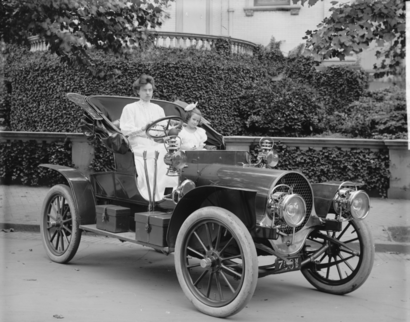
\includegraphics[width=\linewidth]{sample-franklin}
  \caption{1907 Franklin Model D roadster. Photograph by Harris \&
    Ewing, Inc. [Public domain], via Wikimedia
    Commons. (\url{https://goo.gl/VLCRBB}).}
  \Description{A woman and a girl in white dresses sit in an open car.}
\end{figure}

Your figures should contain a caption which describes the figure to the
reader.

Figure captions are placed {\itshape below} the figure.

Every figure should also have a figure description unless it is purely
decorative. These descriptions convey what is in the image to someone
who cannot see it. They are also used by search engine crawlers for
indexing images, and when images cannot be loaded.

A figure description must be unformatted plain text less than 2000
characters long (including spaces). {\bfseries Figure descriptions
  should not repeat the figure caption --- their purpose is to capture
  important information that is not already provided in the caption or
  the main text of the paper.}

\subsection{Full-width Figures}
\label{sec:wide-figures}

An image, or set of images in one figure, that spans the page is created
with the \textbf{figure*} environment, in the same way as a wide table:
\begin{verbatim}
  \begin{figure*}
    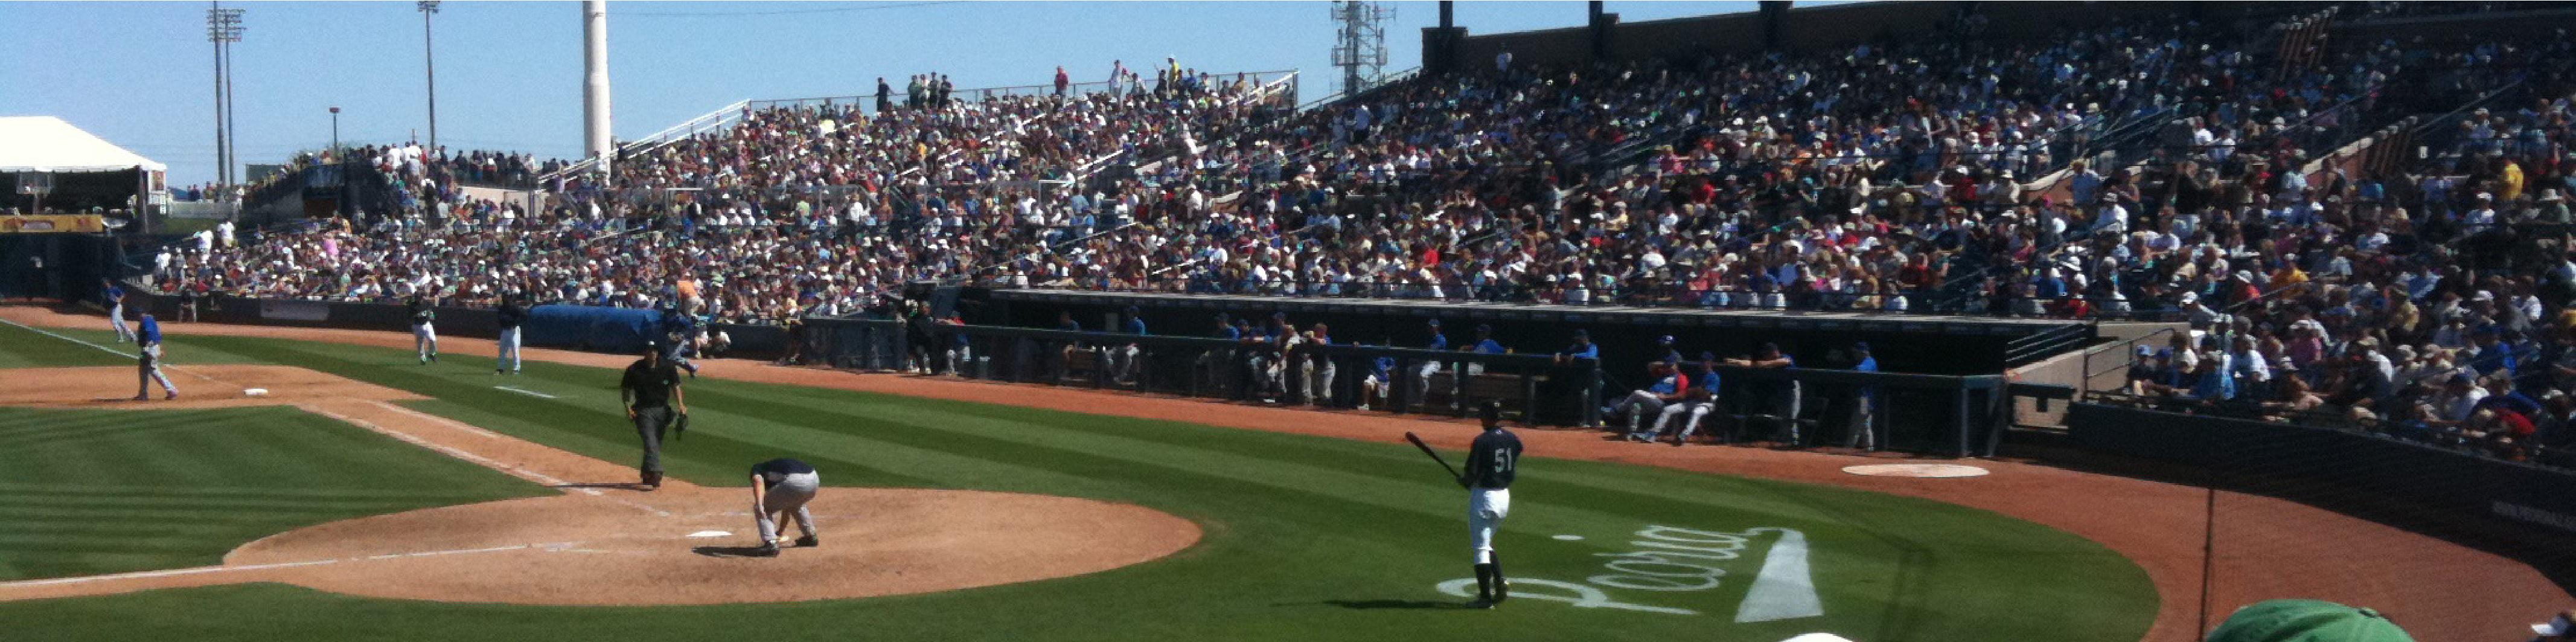
\includegraphics[width=\textwidth]{sampleteaser}
    \caption{figure caption}
    \Description{figure description}
  \end{figure*}
\end{verbatim}

\begin{figure*}
  \centering
  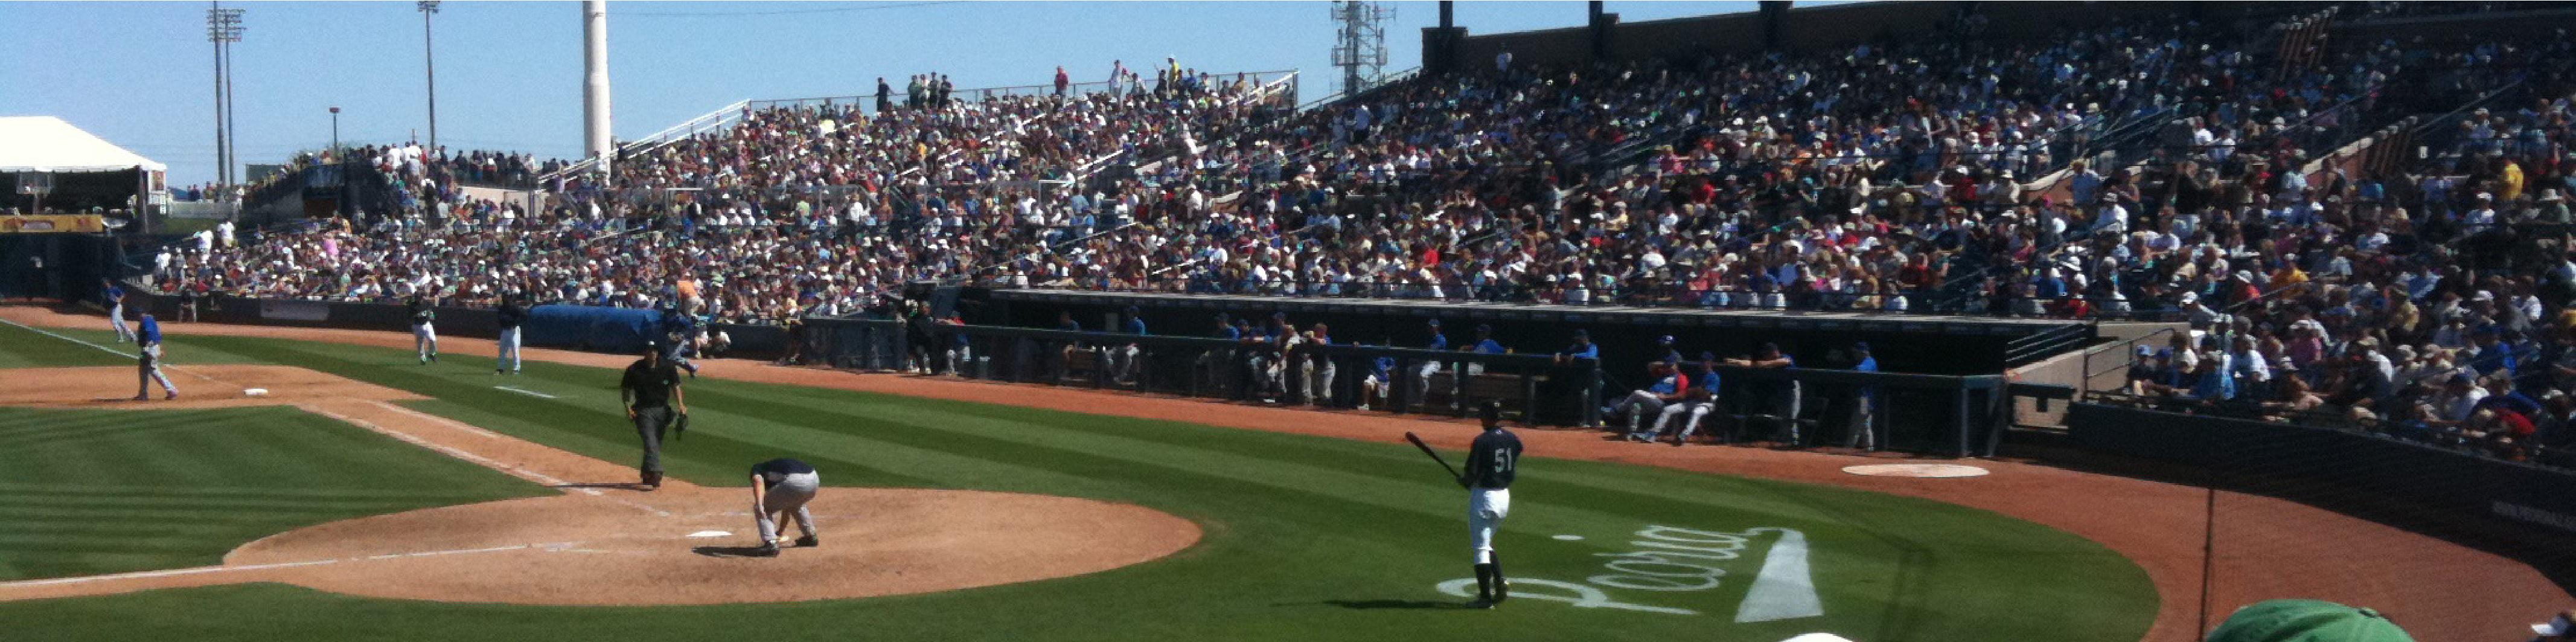
\includegraphics[width=\textwidth]{sampleteaser}
  \caption{Seattle Mariners at Spring Training, 2010.}
  \Description{Enjoying the baseball game from the third-base seats.
    Ichiro Suzuki preparing to bat.}
  \label{fig:teaser}
\end{figure*}

\chapter{Mathematics}
\label{ch:math}

You may want to display math equations in three distinct styles:
inline, numbered or non-numbered display. Each of the three are
discussed in the next sections.

\section{Inline (In-text) Equations}
\label{sec:inline-math}

A formula that appears in the running text is called an inline or
in-text formula. It is produced by the \textbf{math} environment, which
can be invoked with the usual
\texttt{{\char'134}begin\,\ldots{\char'134}end} construction or with the
short form \texttt{\$\,\ldots\$}. You can use any of the symbols and
structures, from $\alpha$ to $\omega$, available in \LaTeX~\cite{Lamport:LaTeX};
this section will simply show a few examples of in-text equations in
context. Notice how this equation:
\begin{math}
  \lim_{n\rightarrow \infty}x=0
\end{math},
set here in in-line math style, looks slightly different when set in
display style. (See next section).

\section{Display Equations}
\label{sec:display-math}

A numbered display equation---one set off by vertical space from the text
and centered horizontally---is produced by the \textbf{equation}
environment. An unnumbered display equation is produced by the
\textbf{displaymath} environment.

Again, in either environment, you can use any of the symbols and
structures available in \LaTeX\@; this section will just give a couple
of examples of display equations in context. First, consider the
equation, shown as an inline equation above:
\begin{equation}
  \label{eq:lim}
  \lim_{n\rightarrow \infty}x=0
\end{equation}
Notice how it is formatted somewhat differently in the
\textbf{displaymath}
environment. Now, we'll enter an unnumbered equation:
\begin{displaymath}
  \sum_{i=0}^{\infty} x + 1
\end{displaymath}
and follow it with another numbered equation:
\begin{equation}
  \label{eq:sum}
  \sum_{i=0}^{\infty}x_i=\int_{0}^{\pi+2} f
\end{equation}
just to demonstrate \LaTeX's able handling of numbering.

\chapter{Citations and Bibliographies}
\label{ch:citations}

The use of \BibTeX\ for the preparation and formatting of one's
references is strongly recommended. Authors' names should be complete
--- use full first names (``Donald E. Knuth'') not initials
(``D. E. Knuth'') --- and the salient identifying features of a
reference should be included: title, year, volume, number, pages,
article DOI, etc.

The bibliography is included in your source document with these two
commands, placed just before the \verb|\end{document}| command:
\begin{verbatim}
  \bibliographystyle{ACM-Reference-Format}
  \bibliography{bibfile}
\end{verbatim}
where ``\verb|bibfile|'' is the name, without the ``\verb|.bib|''
suffix, of the \BibTeX\ file. The class loads the
\texttt{ACM-Reference-Format} style by default.

Citations and references are numbered by default. A small number of
documents use citations and references formatted in the ``author year''
style; for these, pass the \texttt{authoryear} parameter to the
document class:
\begin{verbatim}
  \documentclass[print, authoryear]{thesis}
\end{verbatim}

Some examples follow. A paginated journal article \cite{Abril07}, an
enumerated journal article \cite{Cohen07}, a reference to an entire
issue \cite{JCohen96}, a monograph (whole book) \cite{Kosiur01}, a
monograph/whole book in a series \cite{Harel79}, a divisible-book such
as an anthology or compilation \cite{Editor00} followed by the same
example where only the series is output if the volume number is given
\cite{Editor00a}, a chapter in a divisible book \cite{Spector90}, a
chapter in a divisible book in a series \cite{Douglass98}, a
multi-volume work as book \cite{Knuth97}, a couple of articles in a
proceedings \cite{Andler79, Hagerup1993}, a proceedings article with
all possible elements \cite{Smith10}, an example of an enumerated
proceedings article \cite{VanGundy07}, an informally published work
\cite{Harel78}, a couple of preprints \cite{Bornmann2019,
  AnzarootPBM14}, a doctoral dissertation \cite{Clarkson85}, a master's
thesis \cite{anisi03}, an online document \cite{Thornburg01,
  Ablamowicz07, Poker06}, a video game \cite{Obama08, Novak03, Lee05},
a patent \cite{JoeScientist001}, work accepted for publication
\cite{rous08}, and a few works by a prolific author \cite{SaeediMEJ10,
  SaeediJETC10}. Other cites might contain 'duplicate' DOI and URLs
(some SIAM articles) \cite{Kirschmer:2010:AEI:1958016.1958018}.
Multi-volume works as books \cite{MR781536} and \cite{MR781537}. A
presentation~\cite{Reiser2014}. An article under
review~\cite{Baggett2025}. A couple of citations with DOIs:
\cite{2004:ITE:1009386.1010128,Kirschmer:2010:AEI:1958016.1958018}.
Online citations: \cite{TUGInstmem, Thornburg01, CTANacmart}.
Artifacts: \cite{R} and \cite{UMassCitations}.

\chapter{Conclusion}
\label{ch:conclusion}

This thesis template adapts the ACM article template to the structure of
a thesis. It keeps the typography and the workflow ideas of the original
--- review, print and screen renderings --- while organising the
document by chapter and adding the parts that a thesis requires: a cover
page, a table of contents, lists of figures and tables, an abstract, a
bibliography, and special parts such as the declaration, preface and
acknowledgements.

\section{Further Reading}
\label{sec:further-reading}

For further information, the {\itshape \LaTeX\ User's Guide} and the ACM
template documentation are valuable references.

\section{Ethics and Privacy Statement}
\label{sec:ethics}

This section of your work should discuss the potential societal risks
that might result from its publication. The privacy and ethics statement
should clearly address the broader impacts of the work as it relates to
your interpretation of privacy, fairness, safety, human rights, data
sovereignty, or future misuse, and any benefit/risk trade-off resulting
from the research. We acknowledge that some theses may have minimal
societal risks beyond those considered by institutional review boards,
and the dimensions considered by any review of the study design or
dataset licenses could be provided in this statement.


\backmatter
\bibliography{sample-base,references}

\appendix
\chapter{Supplementary Material}
\label{app:supplementary}

\section{Research Methods}
\label{app:methods}

\subsection{Part One}

Lorem ipsum dolor sit amet, consectetur adipiscing elit. Morbi
malesuada, quam in pulvinar varius, metus nunc fermentum urna, id
sollicitudin purus odio sit amet enim. Aliquam ullamcorper eu ipsum
vel mollis. Curabitur quis dictum nisl. Phasellus vel semper risus, et
lacinia dolor. Integer ultricies commodo sem nec semper.

\subsection{Part Two}

Etiam commodo feugiat nisl pulvinar pellentesque. Etiam auctor sodales
ligula, non varius nibh pulvinar semper. Suspendisse nec lectus non
ipsum convallis congue hendrerit vitae sapien. Donec at laoreet
eros. Vivamus non purus placerat, scelerisque diam eu, cursus
ante. Etiam aliquam tortor auctor efficitur mattis.

\section{Online Resources}
\label{app:resources}

Nam id fermentum dui. Suspendisse sagittis tortor a nulla mollis, in
pulvinar ex pretium. Sed interdum orci quis metus euismod, et sagittis
enim maximus. Vestibulum gravida massa ut felis suscipit
congue. Quisque mattis elit a risus ultrices commodo venenatis eget
dui. Etiam sagittis eleifend elementum.

Nam interdum magna at lectus dignissim, ac dignissim lorem
rhoncus. Maecenas eu arcu ac neque placerat aliquam. Nunc pulvinar
massa et mattis lacinia.


\end{document}
